%%%%%%%%%%%%%%%%%%%%%%%%%%%%%%%%%%%%%%%%%%%%%%%%%%%%%%%%%%%%%%%%%%%%%%%%%%%
% Chapter: Basics
% Falstad examples: examples/basics (generated by falstad/circuits/basics.py)
%%%%%%%%%%%%%%%%%%%%%%%%%%%%%%%%%%%%%%%%%%%%%%%%%%%%%%%%%%%%%%%%%%%%%%%%%%%

%%%%%%%%%%%%%%%%%%%%%%%%%%%%%%%%%%%%%%%%%%%%%%%%%%%%%%%%%%%%%%%%%%%%%%%%%%%
\section{Quantities, Units and Ohm's Law}
%%%%%%%%%%%%%%%%%%%%%%%%%%%%%%%%%%%%%%%%%%%%%%%%%%%%%%%%%%%%%%%%%%%%%%%%%%%
\nsl{This chapter collects the tools that every later chapter uses: the
basic quantities and their units, Ohm's law, Kirchhoff's laws, the voltage
divider, equivalent sources, the LED with its series resistor and the RC
circuit. Most of it is known from the introductory course on electrical
engineering. Here it is repeated with a view to the lab: at the end of the
semester you will build a measurement chain ``From Sensor to Digital
Value''. A resistive sensor sits in a bridge, an instrumentation amplifier
scales the signal to \SIrange{0}{4}{\volt}, a low-pass filter limits the
bandwidth, a sample and hold circuit freezes the value and a 3-bit flash
converter with a resistor ladder turns it into a number that is shown on
LEDs. Every block of this chain is built from the elements of this
chapter.\newline
We also introduce the circuit simulator Falstad (CircuitJS). Every circuit
of the lecture exists as a Falstad file, so you can change values and
watch the effect immediately.\newpage}

\begin{description}
\item[{\rot\bf Quantities and units}]~\\[-\lblskip]
\begin{center}
\resizebox{\linewidth}{!}{%
\begin{tabular}{llll}
\toprule
quantity & symbol & unit & definition \\
\midrule
voltage & $V$ & volt, \si{\volt} & energy per charge, \si{\joule\per\coulomb} \\
current & $I$ & ampere, \si{\ampere} & charge per time, \si{\coulomb\per\second} \\
resistance & $R$ & ohm, \si{\ohm} & $R = V/I$ \\
power & $P$ & watt, \si{\watt} & $P = V\cdot I$ \\
capacitance & $C$ & farad, \si{\farad} & $C = Q/V$ \\
time, frequency & $t$, $f$ & \si{\second}, \si{\hertz} & $f = 1/T$ \\
\bottomrule
\end{tabular}}
\end{center}
\bi
	\ite prefixes: p ($10^{-12}$), n ($10^{-9}$), \textmu{} ($10^{-6}$), m ($10^{-3}$), k ($10^{3}$), M ($10^{6}$)
	\ite useful combination: \si{\volt} / \si{\kilo\ohm} = \si{\milli\ampere}, \si{\milli\ampere} $\cdot$ \si{\kilo\ohm} = \si{\volt}
\ei
\nsl{Calculating with \si{\kilo\ohm}, \si{\milli\ampere} and \si{\volt}
avoids most errors with powers of ten: \SI{5}{\volt} across
\SI{2.2}{\kilo\ohm} gives \SI{2.27}{\milli\ampere} without any exponent.
Voltages are always measured \emph{between two points}. If only one point
is named, the second one is ground (\SI{0}{\volt}). In the diagrams
voltages are drawn as arrows, currents as arrows on the wires; the
direction of an arrow defines the sign, not the physics. A negative result
simply means that the real direction is opposite to the arrow.}
\os{\newpage}

\item[{\rot\bf Ohm's law}]~\\[-\lblskip]
\begin{center}
\begin{circuitikz}[scale=1.2, transform shape]
  \draw (0,0) to[V, invert, l=$V$] (0,3) to[short, i=$I$] (3,3)
        to[R, l=$R$] (3,0) -- (0,0);
\end{circuitikz}
\end{center}
\keyeq{Ohm's law}{$\displaystyle V = R\cdot I \qquad I = \frac{V}{R} \qquad R = \frac{V}{I}$}
\bi
	\ite a resistor is \textbf{linear}: double voltage $\Rightarrow$ double current
	\ite the conductance $G = 1/R$ is measured in siemens, \si{\siemens}
\ei
\nsl{Ohm's law describes resistors, but many other components are
nonlinear: for a diode or an LED the current grows exponentially with the
voltage, so there is no single value $R$. For such components we use a
characteristic curve or a simplified model, for example a constant forward
voltage $V_F$.}
\os{\newpage}

\item[{\rot\bf Power and power rating}]~\\
\keyeq{Power in a resistor}{$\displaystyle P = V\cdot I = I^2\,R = \frac{V^2}{R}$}
\bi
	\ite the power is turned into heat; every resistor has a \textbf{power rating}
	\itee SMD 0603: \SI{0.1}{\watt}, SMD 1206: \SI{0.25}{\watt}, through-hole (0207): \SIrange{0.25}{0.6}{\watt}
	\ite design rule: stay below about \SI{50}{\percent} of the rating
	\ite small signal circuits (\si{\kilo\ohm}, mA) dissipate only mW
	\ite example: \SI{100}{\ohm} at \SI{5}{\volt}: $P = \SI{25}{\volt\squared}/\SI{100}{\ohm} = \SI{250}{\milli\watt}$, too much for a \SI{0.25}{\watt} resistor
\ei
\nsl{The power rating is specified at an ambient temperature of typically
\SI{70}{\celsius}; above that it must be derated. A resistor at its full
rating becomes hot (well above \SI{100}{\celsius}), its value drifts and its
life is shortened. Therefore we keep a safety factor of two. In measurement
circuits the dissipated power matters for another reason: a sensor that
heats itself measures its own temperature. This \emph{self-heating} is the
reason why the sensor current in the capstone task is limited to
\SI{1}{\milli\ampere}.}
\os{\newpage}

\item[{\rot\bf Standard values: the E-series}]~\\[-\lblskip]
\bi
	\ite resistors are not available in every value, but in logarithmic series
	\ite E12 (\SI{10}{\percent} tolerance): 1.0\; 1.2\; 1.5\; 1.8\; 2.2\; 2.7\; 3.3\; 3.9\; 4.7\; 5.6\; 6.8\; 8.2
	\ite E24 (\SI{5}{\percent}) adds: 1.1\; 1.3\; 1.6\; 2.0\; 2.4\; 3.0\; 3.6\; 4.3\; 5.1\; 6.2\; 7.5\; 9.1
	\ite E96 (\SI{1}{\percent}): 96 values per decade, standard for metal film resistors today
	\ite each value exists in every decade: \SI{4.7}{\ohm}, \SI{47}{\ohm}, \ldots, \SI{4.7}{\mega\ohm}
\ei
\nsl{The neighbouring values of a series differ by a constant factor
($10^{1/12}\approx 1.21$ for E12), so that the tolerance bands of
neighbouring values just touch. Today most resistors have a tolerance of
\SI{1}{\percent} even if one uses E12 or E24 values; the coarser series are
simply easier to remember and to keep in stock. A design normally ends with
choosing the next standard value and recalculating the result with it.
Capacitors are usually available in E6 (1.0, 1.5, 2.2, 3.3, 4.7, 6.8).}
\os{\newpage}
\end{description}

%%%%%%%%%%%%%%%%%%%%%%%%%%%%%%%%%%%%%%%%%%%%%%%%%%%%%%%%%%%%%%%%%%%%%%%%%%%
\section{Kirchhoff's Laws and Networks}
%%%%%%%%%%%%%%%%%%%%%%%%%%%%%%%%%%%%%%%%%%%%%%%%%%%%%%%%%%%%%%%%%%%%%%%%%%%
\nsl{Two conservation laws are enough to analyse any network of resistors
and sources: charge is not lost at a node, and energy is not gained on a
closed path. Together with Ohm's law they give as many equations as there
are unknown currents. For the small networks of this lecture we mostly
combine resistors in series and in parallel step by step.\newpage}

\begin{description}
\item[{\rot\bf Kirchhoff's current law (KCL) and voltage law (KVL)}]~\\[-\lblskip]
\begin{center}
\begin{circuitikz}[scale=1.1, transform shape]
  % node with currents
  \draw (0,1.5) to[short, i=$I_1$] (1.8,1.5);
  \draw (1.8,3.3) to[short, i_=$I_2$] (1.8,1.5);
  \draw (1.8,1.5) to[short, i=$I_3$] (3.6,1.5);
  \draw (1.8,1.5) to[short, i=$I_4$] (1.8,-0.3);
  \fill (1.8,1.5) circle (2pt);
  % loop
  \draw (5.5,0) to[V, invert, l=$V_0$] (5.5,3) to[R, l_=$R_1$, v^=$V_1$] (9,3)
        to[R, l=$R_2$, v_=$V_2$] (9,0) -- (5.5,0);
  \draw[->, rwucyandark, thick] (6.7,1.4) arc (150:-150:0.45);
\end{circuitikz}
\end{center}
\bi
	\ite KCL: at every node the sum of incoming currents equals the sum of outgoing currents: $I_1 + I_2 = I_3 + I_4$
	\ite KVL: around every closed loop the sum of voltages is zero: $V_0 = V_1 + V_2$
\ei
\os{\newpage}

\item[{\rot\bf Series and parallel connection}]~\\[-\lblskip]
\begin{center}
\begin{circuitikz}[scale=1.1, transform shape]
  \draw (0,0) node[ocirc]{} to[R, l=$R_1$] (2,0) to[R, l=$R_2$] (4,0) node[ocirc]{};
  \draw (6,0) node[ocirc]{} -- (6.5,0) -- (6.5,0.8) to[R, l=$R_1$] (8.5,0.8) -- (8.5,0) -- (9,0) node[ocirc]{};
  \draw (6.5,0) -- (6.5,-0.8) to[R, l_=$R_2$] (8.5,-0.8) -- (8.5,0);
\end{circuitikz}
\end{center}
\keyeq{Series and parallel}{series: $R = R_1 + R_2$ \hfill parallel: $\displaystyle R = R_1\parallelto R_2 = \frac{R_1 R_2}{R_1+R_2}$\hfill\mbox{}}
\bi
	\ite series: same current, the voltages add up
	\ite parallel: same voltage, the currents add up
	\ite parallel resistance is always smaller than the smallest resistor; $R\parallelto R = R/2$
\ei
\os{\newpage}

\item[{\rot\bf Example: series-parallel network}]~\\[-\lblskip]
\begin{center}
\begin{circuitikz}[scale=1.1, transform shape]
  \draw (0,0) to[V, invert, l=$\SI{12}{\volt}$] (0,3) to[short, i_=$I_1$] (1,3)
        to[R, l=$R_1\ \SI{100}{\ohm}$] (3.4,3) -- (6.4,3);
  \draw (3.4,3) to[short, i_=$I_2$] (3.4,2.3) to[R, l_=$R_2\ \SI{220}{\ohm}$] (3.4,0);
  \draw (6.4,3) to[short, i=$I_3$] (6.4,2.3) to[R, l=$R_3\ \SI{330}{\ohm}$] (6.4,0);
  \draw (0,0) -- (6.4,0);
  \draw (3.4,0) node[ground]{};
  \draw (3.4,3) node[circ]{} node[above]{A};
\end{circuitikz}
\end{center}
\bi
	\ite $R_2\parallelto R_3 = \SI{132}{\ohm}$, total $R = \SI{232}{\ohm}$, $I_1 = \SI{12}{\volt}/\SI{232}{\ohm} = \SI{51.7}{\milli\ampere}$
	\ite $V_A = I_1\cdot\SI{132}{\ohm} = \SI{6.83}{\volt}$; $I_2 = \SI{31.0}{\milli\ampere}$, $I_3 = \SI{20.7}{\milli\ampere}$ (KCL: $I_1 = I_2+I_3$)
\ei
\falstad{network}
\nsl{The procedure is always the same: combine the parallel resistors,
add the series resistor, calculate the total current, then go back and
calculate the node voltage and the branch currents. KCL at node A is a
cheap check of the result. Exercise~\ref{ex:basics-network} looks at the
power of each resistor.}
\os{\newpage}
\end{description}

\exercise{Power in a series-parallel network}\label{ex:basics-network}
Use the network above ($\SI{12}{\volt}$, $R_1=\SI{100}{\ohm}$,
$R_2=\SI{220}{\ohm}$, $R_3=\SI{330}{\ohm}$). All resistors are
\SI{0.25}{\watt} types.
\begin{talist}
\ta Calculate the power dissipated in each resistor and the power delivered by the source.
\ta Which resistor is overloaded? Which rating would you choose instead?
\ta Check the currents and powers in Falstad.
\end{talist}

\begin{solution}
\begin{talist}
\ta $P_1 = I_1^2 R_1 = (\SI{51.7}{\milli\ampere})^2\cdot\SI{100}{\ohm} = \SI{268}{\milli\watt}$,
    $P_2 = V_A^2/R_2 = (\SI{6.83}{\volt})^2/\SI{220}{\ohm} = \SI{212}{\milli\watt}$,
    $P_3 = (\SI{6.83}{\volt})^2/\SI{330}{\ohm} = \SI{141}{\milli\watt}$.
    Source: $P = \SI{12}{\volt}\cdot\SI{51.7}{\milli\ampere} = \SI{621}{\milli\watt} = P_1+P_2+P_3$.
\ta $R_1$ exceeds \SI{0.25}{\watt}; $R_2$ is at \SI{85}{\percent} of its rating, which
    is too hot as well. With the \SI{50}{\percent} rule $R_1$ needs \SI{0.6}{\watt}
    and $R_2$ \SI{0.5}{\watt} (better: \SI{1}{\watt} for $R_1$).
\ta \falstad{network}: \texttt{VA} $=\SI{6.83}{\volt}$; hovering over the resistors
    shows $I_1=\SI{51.7}{\milli\ampere}$, $I_2=\SI{31.0}{\milli\ampere}$,
    $I_3=\SI{20.7}{\milli\ampere}$ and the power of each resistor.
\end{talist}
\end{solution}

%%%%%%%%%%%%%%%%%%%%%%%%%%%%%%%%%%%%%%%%%%%%%%%%%%%%%%%%%%%%%%%%%%%%%%%%%%%
\section{The Voltage Divider}
%%%%%%%%%%%%%%%%%%%%%%%%%%%%%%%%%%%%%%%%%%%%%%%%%%%%%%%%%%%%%%%%%%%%%%%%%%%
\nsl{The voltage divider is the most frequently used circuit in this
lecture. It sets operating points, scales signals, forms the reference
ladder of a flash converter and, with a sensor in one branch, it is half
of a measurement bridge. Its weak point is the load: as soon as current is
drawn from the tap, the output voltage drops.\newpage}

\begin{description}
\item[{\rot\bf Unloaded divider}]~\\[-\lblskip]
\begin{center}
\begin{circuitikz}[scale=0.9, transform shape]
  \draw (0,0) to[V, invert, l=$V_0$] (0,3)
        -- (2,3) to[R, l=$R_1$] (2,1.5)
        to[R, l=$R_2$] (2,0) -- (0,0);
  \draw (2,1.5) to[short, -o] (3.5,1.5);
  \draw (3.5,0) node[ocirc]{} -- (2,0);
  \draw (3.5,1.5) to[open, v^=$\Vout$] (3.5,0);
  \draw (2,0) node[ground]{};
\end{circuitikz}
\end{center}
\bi
	\ite the same current flows through $R_1$ and $R_2$: $I = V_0/(R_1+R_2)$
	\ite the voltages divide in the ratio of the resistances
\ei
\keyeq{Voltage divider}{$\displaystyle \Vout = V_0\,\frac{R_2}{R_1+R_2}$}
\os{\newpage}

\item[{\rot\bf Loaded divider}]~\\[-\lblskip]
\bi
	\ite a load $R_L$ appears in parallel to $R_2$:
	$\displaystyle \Vout = V_0\,\frac{R_2\parallelto R_L}{R_1+R_2\parallelto R_L}$
	\ite seen from the load the divider is a real source with
	$V_\mathrm{th} = V_0\,R_2/(R_1+R_2)$ and $R_\mathrm{th}=R_1\parallelto R_2$
	\ite rule of thumb: $R_L \geq 10\,(R_1\parallelto R_2)$ keeps the error below \SI{10}{\percent}
	\ite for an error below \SI{1}{\percent}: $R_L \geq 100\,(R_1\parallelto R_2)$, or buffer the tap with an op-amp
\ei
\falstad{divider_loaded}
\nsl{Choosing the resistance level of a divider is a trade-off. Small
resistors make the divider stiff against a load, but they draw a large
cross current from the supply and dissipate power. Large resistors save
current, but every load, every leakage current and the input current of
the next stage disturbs the output. In the flash ADC of the capstone task
the reference ladder uses $8\times\SI{1}{\kilo\ohm}$ at \SI{4}{\volt}
($\SI{0.5}{\milli\ampere}$); it is loaded only by comparator inputs, which
draw practically no current.}
\os{\newpage}

\item[{\rot\bf Potentiometer: adjustable divider}]~\\[-\lblskip]
\begin{center}
\begin{circuitikz}[scale=0.9, transform shape]
  \draw (0,0) to[V, invert, l=$V_0$] (0,3) -- (2,3)
        to[pR, n=pot, l_=$R_P$] (2,0) -- (0,0);
  \draw (pot.wiper) to[short, -o] (3.5,1.5);
  \draw (3.5,0) node[ocirc]{} -- (2,0);
  \draw (3.5,1.5) to[open, v^=$\Vout$] (3.5,0);
  \draw (2,0) node[ground]{};
  \draw (6,0) to[V, invert, l=$V_0$] (6,3) -- (8,3) to[R, l=$R_1$] (8,1.9)
        to[pR, n=trim, l_=$R_T$] (8,0.6) to[R, l=$R_2$] (8,-0.5) -- (6,-0.5) -- (6,0);
  \draw (trim.wiper) to[short, -o] (9.3,1.25);
\end{circuitikz}
\end{center}
\bi
	\ite the wiper divides the track: $\Vout = V_0\cdot x$, $x = 0\ldots 1$ (linear taper)
	\ite trimmer between two fixed resistors: fine adjustment over a small range
	\ite the wiper must not carry a large current; load it lightly
\ei
\nsl{A potentiometer is a resistive track with a sliding contact. Panel
potentiometers have a knob, trimmers are adjusted once with a screwdriver.
In the capstone task a trimmer sets the gain of the instrumentation
amplifier so that the full temperature range gives exactly
\SIrange{0}{4.00}{\volt}. Putting the trimmer between two fixed resistors
limits the adjustment range and makes the adjustment much finer: a
\SI{1}{\kilo\ohm} trimmer between two \SI{4.7}{\kilo\ohm} resistors at
\SI{10}{\volt} covers only \SIrange{4.5}{5.5}{\volt}. In Falstad a
potentiometer is found under \emph{Draw $\rightarrow$ Passive Components
$\rightarrow$ Potentiometer}; it gets a slider automatically.}
\os{\newpage}

\item[{\rot\bf Current divider}]~\\[-\lblskip]
\begin{center}
\begin{circuitikz}[scale=1.1, transform shape]
  \draw (0,0) to[I, l=$I$] (0,3) -- (5,3);
  \draw (2.5,3) to[short, i_=$I_1$] (2.5,2.3) to[R, l_=$R_1$] (2.5,0);
  \draw (5,3) to[short, i=$I_2$] (5,2.3) to[R, l=$R_2$] (5,0);
  \draw (0,0) -- (5,0);
\end{circuitikz}
\end{center}
\keyeq{Current divider}{$\displaystyle I_1 = I\,\frac{R_2}{R_1+R_2}\qquad I_2 = I\,\frac{R_1}{R_1+R_2}$}
\bi
	\ite the \textbf{smaller} resistor takes the \textbf{larger} current
	\ite example: \SI{10}{\milli\ampere} into $\SI{1}{\kilo\ohm}\parallelto\SI{4.7}{\kilo\ohm}$:
	$I_1 = \SI{8.25}{\milli\ampere}$, $I_2 = \SI{1.75}{\milli\ampere}$
\ei
\falstad{current_divider}
\os{\newpage}
\end{description}

\exercise{Loaded voltage divider}
A divider with $R_1=R_2=\SI{10}{\kilo\ohm}$ is supplied with $V_0=\SI{10}{\volt}$.
\begin{talist}
\ta Calculate $\Vout$ without load.
\ta Calculate $\Vout$ with a load $R_L=\SI{10}{\kilo\ohm}$.
\ta Check both results in Falstad.
\end{talist}

\begin{solution}
\begin{talist}
\ta $\Vout = \SI{10}{\volt}\cdot \frac{10}{10+10} = \SI{5}{\volt}$.
\ta $R_2\parallelto R_L = \SI{5}{\kilo\ohm}$, so
    $\Vout = \SI{10}{\volt}\cdot\frac{5}{10+5} = \SI{3.33}{\volt}$.
    The load costs one third of the output voltage, because $R_L$ is only
    twice the source resistance $R_\mathrm{th}=\SI{5}{\kilo\ohm}$.
\ta \falstad{divider_loaded}\newline the labels show \texttt{Vout\_open} $=\SI{5.00}{\volt}$
    and \texttt{Vout\_load} $=\SI{3.33}{\volt}$ (move the mouse over the label).
\end{talist}
\end{solution}

%%%%%%%%%%%%%%%%%%%%%%%%%%%%%%%%%%%%%%%%%%%%%%%%%%%%%%%%%%%%%%%%%%%%%%%%%%%
\section{Equivalent Sources and Superposition}
%%%%%%%%%%%%%%%%%%%%%%%%%%%%%%%%%%%%%%%%%%%%%%%%%%%%%%%%%%%%%%%%%%%%%%%%%%%
\nsl{Every linear network of sources and resistors behaves at two
terminals exactly like one ideal voltage source with one series resistor
(Thevenin) or like one ideal current source with one parallel resistor
(Norton). This is the most useful simplification in circuit design: a
bridge half, a sensor with its supply or a divider are replaced by one
source and one resistor, and the effect of the next stage (the load) can
be calculated in one line. The superposition principle is the second tool
for linear networks with several sources.\newpage}

\begin{description}
\item[{\rot\bf Thevenin and Norton equivalent}]~\\[-\lblskip]
\begin{center}
\begin{circuitikz}[scale=0.9, transform shape]
  \draw (0,0) rectangle (2,3);
  \node[align=center] at (1,1.5) {linear\\network};
  \draw (2,2.5) to[short, -o] (2.8,2.5) node[right]{A};
  \draw (2,0.5) to[short, -o] (2.8,0.5) node[right]{B};
  \node at (3.7,1.5) {$\Leftrightarrow$};
  \draw (5.4,0.5) to[V, invert, l_=$V_\mathrm{th}$] (5.4,2.5)
        to[R, l=$R_\mathrm{th}$, -o] (7.8,2.5);
  \draw (5.4,0.5) to[short, -o] (7.8,0.5);
  \node at (8.6,1.5) {$\Leftrightarrow$};
  \draw (10.3,0.5) to[I, l_=$I_\mathrm{N}$] (10.3,2.5) to[short, -o] (12.8,2.5);
  \draw (11.7,0.5) to[R, l_=$R_\mathrm{th}$] (11.7,2.5);
  \draw (10.3,0.5) to[short, -o] (12.8,0.5);
\end{circuitikz}
\end{center}
\bi
	\ite open-circuit voltage: $V_\mathrm{th} = V_\mathrm{oc}$ (nothing connected to A--B)
	\ite short-circuit current: $I_\mathrm{N} = I_\mathrm{sc}$ (A and B shorted)
	\ite internal resistance $R_\mathrm{th} = V_\mathrm{oc}/I_\mathrm{sc}$, or: set all sources to zero (voltage source $\to$ wire, current source $\to$ open) and calculate the resistance between A and B
\ei
\os{\newpage}

\item[{\rot\bf Example: Thevenin equivalent of a divider}]~\\[-\lblskip]
\begin{center}
\begin{circuitikz}[scale=0.9, transform shape]
  \draw (0,0) to[V, invert, l=$\SI{12}{\volt}$] (0,4) -- (2,4)
        to[R, l=$\SI{2.2}{\kilo\ohm}$] (2,2) to[R, l_=$\SI{3.3}{\kilo\ohm}$] (2,0) -- (0,0);
  \draw (2,2) -- (4,2) to[R, l=$R_L\ \SI{1}{\kilo\ohm}$] (4,0) -- (2,0);
  \draw (4,2) node[circ]{} node[above]{$V_L$};
  \node at (6.2,2) {$\Leftrightarrow$};
  \draw (8,0) to[V, invert, l_=$\SI{7.2}{\volt}$] (8,4)
        to[R, l=$\SI{1.32}{\kilo\ohm}$] (11,4) -- (11,3) to[R, l=$R_L\ \SI{1}{\kilo\ohm}$] (11,0) -- (8,0);
  \draw (11,3) node[circ]{} node[left]{$V_L$};
\end{circuitikz}
\end{center}
\bi
	\ite $V_\mathrm{oc} = \SI{12}{\volt}\cdot 3.3/5.5 = \SI{7.2}{\volt}$, \quad
	$I_\mathrm{sc} = \SI{12}{\volt}/\SI{2.2}{\kilo\ohm} = \SI{5.45}{\milli\ampere}$
	\ite $R_\mathrm{th} = \SI{7.2}{\volt}/\SI{5.45}{\milli\ampere} = \SI{1.32}{\kilo\ohm} = \SI{2.2}{\kilo\ohm}\parallelto\SI{3.3}{\kilo\ohm}$
	\ite with $R_L$: $V_L = \SI{7.2}{\volt}\cdot 1/(1+1.32) = \SI{3.10}{\volt}$ in both circuits
\ei
\falstad{thevenin}
\os{\newpage}

\item[{\rot\bf Load line of a real source}]~\\[-\lblskip]
\begin{center}
\begin{tikzpicture}
\begin{axis}[width=11cm, height=5.5cm, xlabel={$I_L$ / mA}, ylabel={$V_L$ / V},
  xmin=0, xmax=6, ymin=0, ymax=8, grid=major, font=\small]
  \addplot[rwuviolet, very thick, domain=0:5.4545] {7.2 - 1.32*x};
  \addplot[rwucyandark, thick, dashed, domain=0:6] {x*1};
  \addplot[only marks, mark=*, mark size=2pt] coordinates {(3.103,3.103)};
  \node[anchor=west, font=\scriptsize] at (axis cs:0.1,7.6) {$V_\mathrm{oc}=\SI{7.2}{\volt}$};
  \node[anchor=south, font=\scriptsize] at (axis cs:5.3,0.3) {$I_\mathrm{sc}$};
  \node[anchor=west, font=\scriptsize] at (axis cs:3.2,3.0) {operating point};
  \node[anchor=west, font=\scriptsize, rwucyandark] at (axis cs:4.6,5.4) {$R_L=\SI{1}{\kilo\ohm}$};
\end{axis}
\end{tikzpicture}
\end{center}
\bi
	\ite the source can deliver every point on the line $V_L = V_\mathrm{th} - R_\mathrm{th}\,I_L$
	\ite the load forces $V_L = R_L\,I_L$; the intersection is the operating point
\ei
\nsl{The load line is the graphical form of the Thevenin equivalent. It
connects the open-circuit voltage on the voltage axis with the
short-circuit current on the current axis. Its slope is $-R_\mathrm{th}$:
the flatter the line, the stiffer the source. The method also works for
nonlinear loads (an LED, a Zener diode): draw the characteristic of the
load into the same diagram and read the intersection. The next chapter
uses it for real voltage sources.}
\os{\newpage}

\item[{\rot\bf Superposition}]~\\[-\lblskip]
\begin{center}
\begin{circuitikz}[scale=1, transform shape]
  \draw (0,0) to[V, invert, l=$V_1\ \SI{12}{\volt}$] (0,3)
        to[R, l=$R_1\ \SI{1}{\kilo\ohm}$] (3.5,3) to[R, l=$R_2\ \SI{2}{\kilo\ohm}$] (7,3)
        to[V, l=$V_2\ \SI{5}{\volt}$] (7,0) -- (0,0);
  \draw (3.5,3) to[R, l=$R_3\ \SI{2}{\kilo\ohm}$] (3.5,0);
  \draw (3.5,3) node[circ]{} node[above]{X};
  \draw (3.5,0) node[ground]{};
\end{circuitikz}
\end{center}
\bi
	\ite in a linear network the effect of all sources is the sum of the effects of each source alone
	\ite the other sources are set to zero: voltage source $\to$ wire, current source $\to$ open
	\ite $V_1$ alone: $V_{X1} = \SI{12}{\volt}\cdot\frac{R_2\parallelto R_3}{R_1+R_2\parallelto R_3} = \SI{6}{\volt}$;
	$V_2$ alone: $V_{X2} = \SI{5}{\volt}\cdot\frac{R_1\parallelto R_3}{R_2+R_1\parallelto R_3} = \SI{1.25}{\volt}$
	\ite both: $V_X = \SI{7.25}{\volt}$ \quad \falstad{superposition}
\ei
\nsl{Superposition is valid only for linear circuits: it fails as soon as
a diode switches or an op-amp clips. It is also not valid for power,
because power is a quadratic function of current. In the lecture it is
used for amplifiers with several inputs, for example the summing amplifier
or an op-amp circuit with an offset voltage at one input.}
\os{\newpage}
\end{description}

\exercise{Thevenin equivalent from open-circuit voltage and short-circuit current}
The divider $\SI{12}{\volt}$, $R_1=\SI{2.2}{\kilo\ohm}$ (top), $R_2=\SI{3.3}{\kilo\ohm}$ (bottom) feeds a load $R_L=\SI{1}{\kilo\ohm}$.
\begin{talist}
\ta Determine $V_\mathrm{oc}$ and $I_\mathrm{sc}$ at the tap and from them $R_\mathrm{th}$.
\ta Calculate $V_L$ with the equivalent circuit.
\ta Which load would reduce the open-circuit voltage by only \SI{5}{\percent}?
\ta Compare the original circuit and the equivalent in Falstad.
\end{talist}

\begin{solution}
\begin{talist}
\ta $V_\mathrm{oc}=\SI{12}{\volt}\cdot 3.3/(2.2+3.3) = \SI{7.2}{\volt}$. With the tap shorted
    no current flows in $R_2$: $I_\mathrm{sc} = \SI{12}{\volt}/\SI{2.2}{\kilo\ohm} = \SI{5.45}{\milli\ampere}$.
    $R_\mathrm{th} = \SI{7.2}{\volt}/\SI{5.45}{\milli\ampere} = \SI{1.32}{\kilo\ohm}$.
\ta $V_L = \SI{7.2}{\volt}\cdot\frac{1}{1+1.32} = \SI{3.10}{\volt}$.
\ta $V_L/V_\mathrm{oc} = R_L/(R_L+R_\mathrm{th}) = 0.95 \Rightarrow R_L = 19\,R_\mathrm{th} = \SI{25.1}{\kilo\ohm}$
    (E12: \SI{27}{\kilo\ohm}).
\ta \falstad{thevenin}: \texttt{VL\_orig} $=$ \texttt{VL\_equiv} $=\SI{3.10}{\volt}$. Replace $R_L$ by
    a wire and hover over it: the short-circuit current is \SI{5.45}{\milli\ampere} in both circuits.
\end{talist}
\end{solution}

\exercise{Superposition}
Use the circuit of the superposition slide.
\begin{talist}
\ta Calculate $V_X$ with superposition.
\ta Check the result with KCL at node X.
\ta How large is the current through $R_2$, and in which direction does it flow?
\ta Check the three cases in Falstad.
\end{talist}

\begin{solution}
\begin{talist}
\ta $V_1$ alone: $R_2\parallelto R_3 = \SI{1}{\kilo\ohm}$, $V_{X1} = \SI{12}{\volt}\cdot 1/2 = \SI{6}{\volt}$.
    $V_2$ alone: $R_1\parallelto R_3 = \SI{0.667}{\kilo\ohm}$, $V_{X2} = \SI{5}{\volt}\cdot 0.667/2.667 = \SI{1.25}{\volt}$.
    $V_X = \SI{7.25}{\volt}$.
\ta $\frac{12-7.25}{1} = \SI{4.75}{\milli\ampere}$ flows in through $R_1$;
    $\frac{7.25}{2} = \SI{3.625}{\milli\ampere}$ flows out through $R_3$ and
    $\frac{7.25-5}{2} = \SI{1.125}{\milli\ampere}$ through $R_2$: $4.75 = 3.625+1.125$ \checkmark
\ta \SI{1.125}{\milli\ampere} from X into the \SI{5}{\volt} source: $V_2$ is charged (absorbs power).
\ta \falstad{superposition}: \texttt{VX1} $=\SI{6.00}{\volt}$, \texttt{VX2} $=\SI{1.25}{\volt}$, \texttt{VX} $=\SI{7.25}{\volt}$.
\end{talist}
\end{solution}

%%%%%%%%%%%%%%%%%%%%%%%%%%%%%%%%%%%%%%%%%%%%%%%%%%%%%%%%%%%%%%%%%%%%%%%%%%%
\section{The LED with Series Resistor}
%%%%%%%%%%%%%%%%%%%%%%%%%%%%%%%%%%%%%%%%%%%%%%%%%%%%%%%%%%%%%%%%%%%%%%%%%%%
\nsl{The light emitting diode is the first nonlinear component of the
lecture and the first task of the lab. It is also the last element of the
capstone chain: the digital value of the flash converter is shown on LEDs,
``exactly the LED and resistor from Task 1''. An LED must never be
connected directly to a voltage source. Its current rises exponentially
with the voltage, so a few tenths of a volt make the difference between
dark and destroyed. The series resistor turns the voltage source into a
(rough) current source and sets the current.\newpage}

\begin{description}
\item[{\rot\bf LED characteristic}]~\\[-\lblskip]
\begin{center}
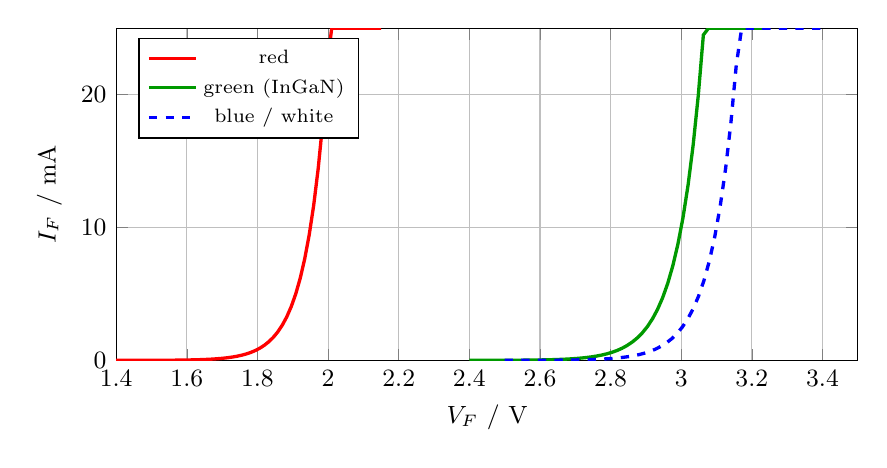
\begin{tikzpicture}
\begin{axis}[width=11cm, height=5.8cm, xlabel={$V_F$ / V}, ylabel={$I_F$ / mA},
  xmin=1.4, xmax=3.5, ymin=0, ymax=25, grid=major, font=\small,
  legend pos=north west, legend style={font=\scriptsize}]
  \addplot[red, very thick, domain=1.4:2.15, samples=60] {min(25, 10*exp((x-1.95)/0.06))};
  \addplot[green!60!black, very thick, domain=2.4:3.25, samples=60] {min(25, 10*exp((x-3.0)/0.07))};
  \addplot[blue, very thick, dashed, domain=2.5:3.4, samples=60] {min(25, 10*exp((x-3.1)/0.07))};
  \legend{red, green (InGaN), blue / white}
\end{axis}
\end{tikzpicture}
\end{center}
\bi
	\ite below a threshold almost no current, above it the current rises steeply
	\ite simple model: constant forward voltage $V_F$ at the operating current
\ei
\os{\newpage}

\item[{\rot\bf Forward voltage and current}]~\\[-\lblskip]
\begin{center}
\begin{tabular}{lll}
\toprule
colour & material & $V_F$ at \SIrange{10}{20}{\milli\ampere} \\
\midrule
infrared & GaAs & \SIrange{1.2}{1.5}{\volt} \\
red & AlGaInP & \SIrange{1.8}{2.1}{\volt} \\
yellow, orange & AlGaInP & \SIrange{2.0}{2.2}{\volt} \\
green (classic, yellow-green) & GaP & \SIrange{2.1}{2.4}{\volt} \\
green (true green), blue, white & InGaN & \SIrange{2.8}{3.4}{\volt} \\
\bottomrule
\end{tabular}
\end{center}
\bi
	\ite standard \SI{3}{\milli\meter}/\SI{5}{\milli\meter} LEDs: $I_F \leq \SI{20}{\milli\ampere}$; modern LEDs are clearly visible at \SIrange{2}{5}{\milli\ampere}
	\ite reverse voltage only about \SI{5}{\volt}: an LED is not a rectifier
\ei
\nsl{The forward voltage grows with the photon energy, i.e.\ it is
higher for shorter wavelengths: red needs less than \SI{2}{\volt}, blue and
white (a blue LED with a phosphor) need about \SI{3}{\volt}. This matters
for a \SI{3.3}{\volt} supply, where a blue LED leaves only a few hundred
millivolts for the series resistor and the current depends strongly on the
spread of $V_F$. The forward voltage also decreases by about
\SI{2}{\milli\volt\per\kelvin}, so an LED without a resistor heats up,
draws more current and heats up further.}
\os{\newpage}

\item[{\rot\bf Dimensioning the series resistor}]~\\[-\lblskip]
\begin{center}
\begin{circuitikz}[scale=1.1, transform shape]
  \draw (0,0) to[V, invert, l=$V_S$] (0,4) to[short, i=$I_F$] (2.5,4)
        to[R, l=$R$, v_=$V_R$] (2.5,2)
        to[leD, l=$V_F$] (2.5,0) -- (0,0);
  \draw (2.5,0) node[ground]{};
\end{circuitikz}
\end{center}
\keyeq{LED series resistor}{$\displaystyle R = \frac{V_S - V_F}{I_F}\qquad P_R = (V_S-V_F)\cdot I_F$}
\bi
	\ite example: $V_S = \SI{5}{\volt}$, red LED $V_F = \SI{2.0}{\volt}$, $I_F = \SI{10}{\milli\ampere}$:
	$R = \SI{300}{\ohm}$ $\Rightarrow$ E12: \SI{330}{\ohm}, $I_F = \SI{9.1}{\milli\ampere}$, $P_R = \SI{27}{\milli\watt}$
\ei
\os{\newpage}

\item[{\rot\bf Design recipe}]~\\
\designcard{LED with series resistor}{
\begin{enumerate}\itemsep 0pt
	\item take $V_F$ from the datasheet at the desired current (or the table: red \SI{2.0}{\volt}, blue/white \SI{3.0}{\volt})
	\item choose $I_F$: \SIrange{2}{10}{\milli\ampere} for an indicator, check the maximum current of the driver
	\item $R = (V_S - V_F)/I_F$, round \textbf{up} to the next E12/E24 value
	\item recalculate $I_F$ and check $P_R = I_F^2 R$ against the rating
\end{enumerate}}
\bi
	\ite rounding up keeps the current below the target, which protects LED and driver
	\ite the larger $V_S - V_F$, the less $I_F$ depends on the spread of $V_F$
\ei
\nsl{The last point explains why the resistor works as a current source:
the current is $I_F = (V_S-V_F)/R$. If $V_F$ changes by \SI{0.1}{\volt},
the current changes by \SI{0.1}{\volt}/$R$, which is \SI{3}{\percent} at
$V_S=\SI{5}{\volt}$ but \SI{8}{\percent} at \SI{3.3}{\volt} for a red LED.
For a blue LED at \SI{3.3}{\volt} the scheme hardly works any more; a
real current source (chapter Sources) is better.}
\os{\newpage}

\item[{\rot\bf Driving an LED from a logic output}]~\\[-\lblskip]
\begin{center}
\begin{circuitikz}[scale=1, transform shape]
  \node[draw, thick, minimum width=1.8cm, minimum height=1cm, align=center, font=\small] (g1) at (0,3) {logic\\output};
  \draw (g1.east) to[R, l=$R$] (3.4,3) to[leD] (3.4,1) node[ground]{};
  \node[font=\small] at (1.5,0) {source: high = on};
  \draw (8.6,4.2) node[vcc]{$+\SI{5}{\volt}$} to[R, l=$R$] (8.6,2.6) to[leD] (8.6,1) -- (7.2,1);
  \node[draw, thick, minimum width=1.8cm, minimum height=1cm, align=center, font=\small, anchor=east] (g2) at (7.2,1) {logic\\output};
  \node[font=\small] at (7.4,0) {sink: low = on};
\end{circuitikz}
\end{center}
\bi
	\ite a logic output is a switch to $V_S$ or to ground with an output resistance of some \SI{10}{\ohm}
	\ite 74HC at \SI{5}{\volt}: $\pm\SI{4}{\milli\ampere}$ with guaranteed levels, absolute maximum \SI{25}{\milli\ampere} per pin
	\ite microcontrollers: some mA per pin and a limit for the whole port
	\ite \SI{330}{\ohm} at \SI{5}{\volt} gives about \SI{9}{\milli\ampere}, \SI{1}{\kilo\ohm} about \SI{3}{\milli\ampere}
\ei
\falstad{led_resistor}
\nsl{A CMOS output stage consists of a p-channel transistor to the supply
and an n-channel transistor to ground. Each acts like a resistor of some
\SI{10}{\ohm} to \SI{50}{\ohm} when it is switched on. With an LED current
of a few milliampere the output voltage therefore differs by only
\SIrange{0.1}{0.3}{\volt} from the rail, and the simple formula still
applies. The LED can be connected to ground (the output \emph{sources} the
current, the LED is on at high level) or to the supply (the output
\emph{sinks} the current, the LED is on at low level). Older TTL outputs
can sink much more current than they can source; that is why many
datasheets and old circuits connect LEDs to the supply. In the capstone
task the three bits of the encoder drive three LEDs to ground. The Falstad
example uses ideal logic outputs, so the full \SI{5}{\volt} is available.}
\os{\newpage}
\end{description}

\exercise{LED on a \SI{5}{\volt} logic output}\label{ex:basics-led}
A red LED ($V_F=\SI{2.0}{\volt}$ at \SI{10}{\milli\ampere}) is to be driven by a \SI{5}{\volt} logic output.
\begin{talist}
\ta Calculate the series resistor for \SI{10}{\milli\ampere} and choose an E12 value.
\ta Calculate the actual current and the power in the resistor.
\ta The same LED is to be driven from a \SI{3.3}{\volt} microcontroller pin with at most \SI{4}{\milli\ampere}. Choose the resistor.
\ta Falstad uses an LED model with $V_F\approx\SI{1.8}{\volt}$. Which current does the simulation show with \SI{330}{\ohm}?
\end{talist}

\begin{solution}
\begin{talist}
\ta $R = (\SI{5}{\volt}-\SI{2.0}{\volt})/\SI{10}{\milli\ampere} = \SI{300}{\ohm}$; rounded up to E12: \SI{330}{\ohm}.
\ta $I_F = \SI{3.0}{\volt}/\SI{330}{\ohm} = \SI{9.1}{\milli\ampere}$, $P_R = \SI{3.0}{\volt}\cdot\SI{9.1}{\milli\ampere} = \SI{27}{\milli\watt}$:
    any resistor will do, even SMD 0402.
\ta $R \geq (\SI{3.3}{\volt}-\SI{2.0}{\volt})/\SI{4}{\milli\ampere} = \SI{325}{\ohm}$, again \SI{330}{\ohm}
    ($I_F = \SI{3.9}{\milli\ampere}$; $V_F$ is a bit lower at this current, so the real current is slightly higher).
\ta \falstad{led_resistor}: \texttt{VLED} $=\SI{1.78}{\volt}$, so $I_F = (5-1.78)\,\si{\volt}/\SI{330}{\ohm} = \SI{9.76}{\milli\ampere}$
    (hover over the resistor). Use the slider to see how the current changes with $R$.
\end{talist}
\end{solution}

%%%%%%%%%%%%%%%%%%%%%%%%%%%%%%%%%%%%%%%%%%%%%%%%%%%%%%%%%%%%%%%%%%%%%%%%%%%
\section{Capacitor and RC Circuits}
%%%%%%%%%%%%%%%%%%%%%%%%%%%%%%%%%%%%%%%%%%%%%%%%%%%%%%%%%%%%%%%%%%%%%%%%%%%
\nsl{Capacitors store charge. In this lecture they appear as decoupling
capacitors at every supply pin, in filters, in the hold capacitor of the
sample and hold circuit and as the reason for every delay. The RC circuit
is the simplest dynamic circuit; its exponential response and its time
constant $\tau = RC$ appear again and again.\newpage}

\begin{description}
\item[{\rot\bf The capacitor}]~\\[-\lblskip]
\bi
	\ite charge proportional to voltage: $Q = C\cdot V$
	\ite current = change of charge: $\displaystyle I = C\,\frac{dV}{dt}$
	\itee the voltage across a capacitor cannot jump (that would need an infinite current)
	\itee DC: once charged, no current flows (open circuit)
	\ite energy: $E = \frac{1}{2}\,C V^2$
	\ite types: ceramic (\si{\pico\farad} to \SI{100}{\micro\farad}; C0G stable, X7R voltage dependent), film (precise, for filters and hold capacitors), electrolytic (large, polarized)
\ei
\nsl{The relation $I = C\,dV/dt$ is the capacitor's counterpart of Ohm's
law. A constant current charges a capacitor linearly:
\SI{1}{\milli\ampere} into \SI{1}{\micro\farad} gives
\SI{1}{\volt\per\milli\second}. This is used in integrators and ramp
generators. Ceramic capacitors of type X7R or Y5V lose a large part of
their capacitance with DC voltage and temperature; for filters and the
hold capacitor of a sample and hold circuit use C0G (NP0) ceramic or film
capacitors.}
\os{\newpage}

\item[{\rot\bf Charging through a resistor}]~\\[-\lblskip]
\begin{center}
\begin{circuitikz}[scale=1.1, transform shape]
  \draw (0,0) to[sqV, l=$V_\mathrm{in}$] (0,3) to[short, i=$I$] (0.8,3) to[R, l=$R$] (3.5,3)
        to[C, l=$C$] (3.5,0) -- (0,0);
  \draw (3.5,0) node[ground]{};
  \draw (3.5,3) node[circ]{} node[above right]{$V_C$};
\end{circuitikz}
\end{center}
\keyeq{RC charging and discharging}{$\displaystyle V_C(t) = V_0\left(1 - e^{-t/\tau}\right)\qquad
V_C(t) = V_0\,e^{-t/\tau}\qquad \tau = R\,C$}
\bi
	\ite step of $V_0$ at the input; the current $I=(V_\mathrm{in}-V_C)/R$ decreases as $V_C$ rises
	\ite time to reach a voltage $V_1$: $t = \tau\,\ln\frac{V_0}{V_0-V_1}$
\ei
\os{\newpage}

\item[{\rot\bf The time constant}]~\\[-\lblskip]
\begin{center}
\begin{tikzpicture}
\begin{axis}[width=11.5cm, height=5.8cm, xlabel={$t$ / s}, ylabel={$V$ / V},
  xmin=0, xmax=1, ymin=-0.2, ymax=5.6, grid=major, font=\small,
  legend style={font=\scriptsize, at={(0.98,0.5)}, anchor=east}]
  \addplot[rwucyandark, thick, const plot] coordinates {(0,5) (0.5,5) (0.5,0) (1,0)};
  \addplot[rwuviolet, very thick, domain=0:0.5, samples=80] {5*(1-exp(-x/0.1))};
  \addplot[rwuviolet, very thick, domain=0.5:1, samples=80, forget plot] {4.966*exp(-(x-0.5)/0.1)};
  \addplot[black, dashed, domain=0:0.1] {50*x};
  \addplot[only marks, mark=*, mark size=1.5pt] coordinates {(0.1,3.16) (0.5,4.97) (0.6,1.83)};
  \legend{$V_\mathrm{in}$, $V_C$}
  \node[anchor=west, font=\scriptsize] at (axis cs:0.11,3.0) {$\tau$: \SI{63}{\percent}};
  \node[anchor=north, font=\scriptsize] at (axis cs:0.45,4.8) {$5\tau$: \SI{99.3}{\percent}};
  \node[anchor=west, font=\scriptsize] at (axis cs:0.61,1.9) {\SI{37}{\percent}};
\end{axis}
\end{tikzpicture}
\end{center}
\bi
	\ite after $\tau$: \SI{63}{\percent}, after $3\tau$: \SI{95}{\percent}, after $5\tau$: \SI{99.3}{\percent} (``settled'')
	\ite the tangent at $t=0$ reaches the final value after exactly $\tau$
	\ite example $R=\SI{10}{\kilo\ohm}$, $C=\SI{10}{\micro\farad}$: $\tau = \SI{0.1}{\second}$ \quad \falstad{rc_charging}
\ei
\nsl{How long one has to wait depends on the required accuracy. Settling
to within \SI{1}{\percent} takes $4.6\,\tau$, to within half an LSB of an
$n$-bit converter $\tau\ln(2^{n+1})$: $2.8\,\tau$ for the 3-bit converter
of the capstone task, but $9\,\tau$ for a 12-bit converter. This is the
reason why the acquisition time of a sample and hold circuit is specified
together with an accuracy.}
\os{\newpage}

\item[{\rot\bf Preview: the RC low-pass}]~\\[-\lblskip]
\begin{center}
\begin{circuitikz}[scale=1, transform shape]
  \draw (0,2) node[ocirc]{} to[R, l=$R$] (2.5,2) to[short, -o] (4,2);
  \draw (2.5,2) to[C, l=$C$] (2.5,0);
  \draw (0,0) node[ocirc]{} -- (4,0) node[ocirc]{};
  \draw (0,2) to[open, v=$\Vin$] (0,0);
  \draw (4,2) to[open, v^=$\Vout$] (4,0);
\end{circuitikz}
\quad
\begin{tikzpicture}
\begin{semilogxaxis}[width=7cm, height=4.5cm, xlabel={$f/f_c$}, ylabel={$|\Vout/\Vin|$},
  xmin=0.01, xmax=100, ymin=0, ymax=1.1, grid=major, font=\scriptsize]
  \addplot[rwuviolet, very thick, domain=0.01:100, samples=100] {1/sqrt(1+x^2)};
  \addplot[only marks, mark=*, mark size=1.5pt] coordinates {(1,0.707)};
\end{semilogxaxis}
\end{tikzpicture}
\end{center}
\keyeq{Cut-off frequency}{$\displaystyle f_c = \frac{1}{2\pi R C}\qquad \left|\frac{\Vout}{\Vin}\right| = \frac{1}{\sqrt{1+(f/f_c)^2}}$}
\bi
	\ite at $f_c$ the amplitude drops to $1/\sqrt{2} = 0.707$ ($-\SI{3}{\decibel}$), phase $-\ang{45}$
	\ite example: \SI{1.6}{\kilo\ohm}, \SI{100}{\nano\farad}: $f_c = \SI{995}{\hertz}$ \quad \falstad{rc_lowpass}
\ei
\nsl{For slow signals the capacitor follows the input; for fast signals
it cannot charge in time and the output amplitude decreases. Above $f_c$
the amplitude falls by a factor of 10 per decade of frequency
(\SI{-20}{\decibel} per decade). In the capstone task an anti-aliasing
low-pass with $f_c\approx\SI{2.5}{\hertz}$ precedes the sample and hold
circuit that samples at \SI{5}{\hertz}; with $C=\SI{10}{\micro\farad}$ this
needs $R = 1/(2\pi\cdot\SI{2.5}{\hertz}\cdot\SI{10}{\micro\farad}) =
\SI{6.4}{\kilo\ohm}$, E24: \SI{6.2}{\kilo\ohm} ($f_c=\SI{2.57}{\hertz}$).
The chapter on active filters treats filters in detail. The RC low-pass
in the Falstad example is driven with \SI{1}{\kilo\hertz}, almost exactly
$f_c$: the output amplitude is \SI{0.705}{\volt} for an input amplitude of
\SI{1}{\volt}, and the output lags by about a quarter period.}
\os{\newpage}
\end{description}

\exercise{RC charging}
A capacitor $C=\SI{10}{\micro\farad}$ is charged through $R=\SI{10}{\kilo\ohm}$ from a square wave
that switches between \SI{0}{\volt} and \SI{5}{\volt} at \SI{1}{\hertz}.
\begin{talist}
\ta Calculate $\tau$ and $V_C$ after $\tau$ and after \SI{0.5}{\second}.
\ta After which time does $V_C$ reach \SI{4}{\volt}?
\ta To which voltage does $C$ discharge \SI{0.1}{\second} after the falling edge?
\ta Read the values from the Falstad scope.
\end{talist}

\begin{solution}
\begin{talist}
\ta $\tau = \SI{10}{\kilo\ohm}\cdot\SI{10}{\micro\farad} = \SI{0.1}{\second}$.
    $V_C(\tau) = \SI{5}{\volt}\,(1-e^{-1}) = \SI{3.16}{\volt}$;
    $V_C(\SI{0.5}{\second}) = V_C(5\tau) = \SI{5}{\volt}\,(1-e^{-5}) = \SI{4.97}{\volt}$.
\ta $t = \tau\ln\frac{5}{5-4} = \SI{0.1}{\second}\cdot\ln 5 = \SI{0.161}{\second}$.
\ta The discharge starts at \SI{4.97}{\volt}: $V_C = \SI{4.97}{\volt}\cdot e^{-1} = \SI{1.83}{\volt}$.
\ta \falstad{rc_charging}: the scope shows \SI{3.16}{\volt} at \SI{0.1}{\second},
    \SI{4}{\volt} at \SI{0.161}{\second}, \SI{4.97}{\volt} at the falling edge and
    \SI{1.83}{\volt} \SI{0.1}{\second} later.
\end{talist}
\end{solution}

%%%%%%%%%%%%%%%%%%%%%%%%%%%%%%%%%%%%%%%%%%%%%%%%%%%%%%%%%%%%%%%%%%%%%%%%%%%
\section{Working with Falstad}
%%%%%%%%%%%%%%%%%%%%%%%%%%%%%%%%%%%%%%%%%%%%%%%%%%%%%%%%%%%%%%%%%%%%%%%%%%%
\nsl{Falstad's circuit simulator (CircuitJS) runs in the browser and needs
no installation \cite{falstad}. It simulates the circuit continuously and
shows the voltages as colours and the currents as moving dots, which makes
it ideal for getting a feeling for a circuit. It is not a replacement for
SPICE: its models are simple (the op-amp has no bandwidth limit by
default, transistors have no capacitances) and it cannot print exact
plots. For the circuits of this lecture it is accurate enough, and every
example has been checked against the hand calculation.\newpage}

\begin{description}
\item[{\rot\bf Opening and building circuits}]~\\[-\lblskip]
\bi
	\ite \url{https://www.falstad.com/circuit/circuitjs.html}
	\ite open an example: click its Falstad box in the script, or \emph{File $\rightarrow$ Import From Text} and paste the content of \texttt{examples/basics/*.txt}
	\ite new circuit: \emph{Circuits $\rightarrow$ Blank Circuit}
	\ite place elements: \emph{Draw} menu or right click; frequent ones have shortcuts (\texttt{r} resistor, \texttt{c} capacitor, \texttt{w} wire, \texttt{g} ground)
	\ite drag to place, double click to edit values (\texttt{4.7k}, \texttt{100n}, \texttt{10u} are accepted)
	\ite save your work: \emph{File $\rightarrow$ Export As Text} or \emph{Export As Link}
\ei
\os{\newpage}

\item[{\rot\bf Pitfalls when drawing}]~\\[-\lblskip]
\bi
	\ite wires connect \textbf{only at their end points}: a wire passing over a terminal is not connected; split the wire there
	\ite unconnected terminals are shown as red dots
	\ite every circuit needs a ground (or a source that defines the potential)
	\ite \emph{labeled nodes} (\emph{Draw $\rightarrow$ Wiring $\rightarrow$ Labeled Node}) with the same name are connected without a wire, and their name can be used for scopes
	\ite ``singular matrix'': usually a floating node or two ideal voltage sources in parallel
\ei
\nsl{Most errors in self-drawn circuits come from the first rule. A wire
that runs over the end of a resistor looks connected, but it is not. Check
the dots: a junction of three or more wires is drawn with a large dot.
Moving an element with the mouse shows which wires follow it.}
\os{\newpage}

\item[{\rot\bf Measuring}]~\\[-\lblskip]
\bi
	\ite hover the mouse over an element: the bottom right corner shows voltage, current and power
	\ite hover over a labeled node: its voltage to ground
	\ite voltage colours: green positive, red negative, grey zero; yellow dots: current
	\ite scope: right click on an element $\rightarrow$ \emph{View in New Scope}; right click on a scope for settings (scale, several traces, \emph{Max Scale})
	\ite sliders: \emph{Edit} dialog of an element, check \emph{Show slider}; the examples have sliders for the values worth changing
	\ite simulation speed: slider on the right; the time step is in \emph{Options $\rightarrow$ Other Options}
\ei
\nsl{The examples of this lecture are generated by a Python program that
also simulates them and asserts the numbers quoted in this script. When
you open an example, compare the displayed values with the solution of the
exercise. If they differ, check the time: circuits with capacitors need a
few time constants before they reach their final state.\newline
Example: open \texttt{led\_resistor}. Hover over the label \texttt{VLED} to
read the forward voltage (\SI{1.78}{\volt}), hover over the resistor to read
the current (\SI{9.76}{\milli\ampere}), and move the slider to change the
resistor. The two LEDs on the right are driven by inverters and blink in
turn: one is connected as a current source, one as a current sink.}
\os{\newpage}
\end{description}

%%% Local Variables:
%%% mode: latex
%%% TeX-master: "docu"
%%% End:
